\let\lesson\undefined
\newcommand{\lesson}{\phantomlesson{Bài 14: Moment lực. Điều kiện cân bằng của vật.}}
\chapter[Moment lực - Điều kiện cân bằng của vật]{Moment lực - Điều kiện cân bằng của vật}
\setcounter{section}{0}
\section{Lý thuyết}
\subsection{Moment lực}
Moment lực đối với một trục quay là đại lượng đặc trưng cho tác dụng làm quay của lực và được đo bằng tích của lực với cánh tay đòn của nó:
\begin{equation*}
	M = F\cdot d \label{eq1}
\end{equation*}
trong đó: 
\begin{itemize}
	\item $M$ là moment lực ($\si{\newton\cdot\meter}$), 
	\item $F$ là lực đang xét ($\si{\newton}$),
	\item $d$ là cánh tay đòn của lực $F$ ($\si{\meter}$).
\end{itemize}
\manatip{
Cánh tay đòn của lực là khoảng cách từ trục quay đến giá của lực.
\begin{center}
	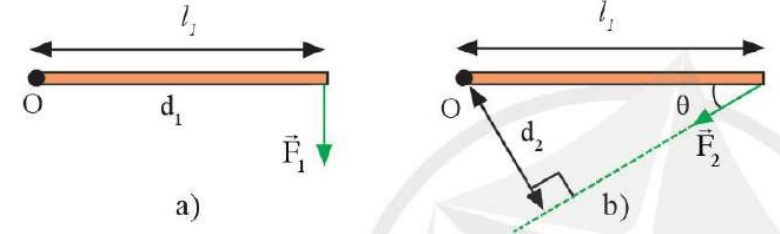
\includegraphics[scale=0.7]{../figs/VN10-2023-PH-TP023-1}
\end{center}
}
\subsection{Điều kiện cân bằng của vật rắn}
\subsubsection{Quy tắc moment lực}
Muốn cho một vật có trục quay cố định ở trạng thái cân bằng (không chuyển động quay) thì tổng các moment lực có xu hướng làm vật quay theo chiều kim đồng hồ phải bằng tổng các moment lực có xu hướng làm vật quay ngược chiều kim đồng hồ.

\begin{center}
	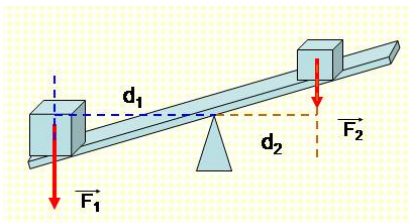
\includegraphics[scale=0.5]{../figs/VN10-PH-21-L-016-2-V2-01.png}
\end{center}
\begin{equation*}
	M_1+M_2+... = M'_1+M'_2+... 
\end{equation*}
%
\begin{equation*}
	F_1\cdot d_1+F_2\cdot d_2 + ... = F'_1\cdot d'_1 + F'_2\cdot d'_2+...
\end{equation*}
\luuy{Quy tắc moment lực còn được áp dụng cho cả trường hợp một vật không có trục quay cố định nếu như trong một tình huống cụ thể nào đó ở vật xuất hiện trục quay tức thời.}
\subsection{Điều kiện cân bằng tổng quát của vật rắn}
Khi vật rắn ở trạng thái cân bằng, lực tác dụng vào vật phải có hai điều kiện sau:
\begin{itemize}
	\item Lực tổng hợp tác dụng lên vật bằng không
	$$\vec{F}_1+\vec{F}_2+\dots+\vec{F}_n=\vec{0}.$$
	\item Tổng moment của các lực làm vật quay theo chiều kim đồng hồ bằng tổng moment của các lực làm vật quay theo chiều ngược lại
	$$M_1+M_2+\dots=M'_1+M'_2+\dots.$$
\end{itemize}
\luuy{Trong điều kiện về moment lực, ta cần quy ước các moment lực có xu hướng làm vật quay theo một chiều có giá trị dương. Từ đó, các moment lực có xu hướng làm vật quay theo chiều ngược với chiều dương quy ước sẽ có giá trị âm.}
\subsection{Ngẫu lực. Moment ngẫu lực}
\subsubsection{Ngẫu lực}
Ngẫu lực là hệ hai lực song song, ngược chiều, có độ lớn bằng nhau và cùng tác dụng vào một vật.
\subsubsection{Tác dụng của ngẫu lực đối với một vật rắn}
\textbf{Trường hợp vật không có trục quay cố định (vật tự do)}

Dưới tác dụng của ngẫu lực:
\begin{itemize}
	\item  Vật sẽ quay quanh trục đi qua trọng tâm và vuông góc với mặt phẳng chứa ngẫu lực.
	\item Trọng tâm đứng yên. Trục quay đi qua trọng tâm không chịu lực tác dụng.
	\begin{center}
		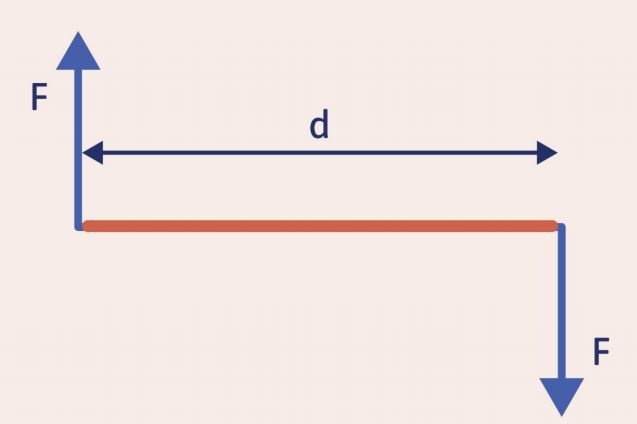
\includegraphics[scale=0.4]{../figs/VN10-PH-25-L-020-1-V2-01.JPG}
	\end{center}	
\end{itemize}
\textbf{Trường hợp vật có trục quay cố định}

Dưới tác dụng của ngẫu lực:
\begin{itemize}
	\item  Vật sẽ quay quanh trục cố định của nó. 
	\item Nếu trục quay không đi qua trọng tâm thì trọng tâm sẽ chuyển động tròn xung quanh trục quay. Khi ấy, vật có xu hướng chuyển động li tâm nên tác dụng lực vào trục quay.
	\item Khi chế tạo các bộ phận quay của máy móc phải làm cho trục quay đi qua trọng tâm của nó.
	\begin{center}
		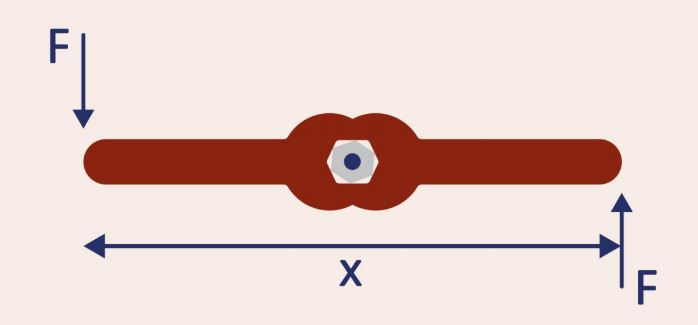
\includegraphics[scale=0.4]{../figs/VN10-PH-25-L-020-1-V2-02.JPG}
	\end{center}
\end{itemize}

\subsubsection{Moment của ngẫu lực}
Đối với các trục quay vuông góc với mặt phẳng chứa ngẫu lực thì moment của ngẫu lực không phụ thuộc vào vị trí trục quay và luôn luôn có giá trị: 
\begin{equation*}
	M=F_1d_1+F_2d_2=F(d_1+d_2)=F\cdot d
\end{equation*}
trong đó:
\begin{itemize}
	\item $F_1=F_2=F$ là độ lớn của mỗi lực ($\si{\newton}$);
	\item $d_1+d_2=d$ là khoảng cách giữa hai giá của ngẫu lực và được gọi là cánh tay đòn của ngẫu lực ($\si{\meter}$);
	\item $M$ là moment của ngẫu lực ($\si{\newton\cdot\meter}$).
\end{itemize}

\section{Mục tiêu bài học - Ví dụ minh họa}
\begin{dang}{Ghi nhớ khái niệm moment lực, công thức tính moment lực}
	\viduii{1}{Đơn vị của moment lực $M = F \cdot d$ là
		\begin{mcq}(4)
			\item $\si{\meter/\second}.$	
			\item $\si{\newton\cdot\meter}.$
			\item $\si{\kilogram\cdot\meter}.$
			\item $\si{\newton\cdot\kilogram}.$
		\end{mcq}
	}
	{	\hide{	\begin{equation*}
				M = F\cdot d, \label{eq1}
			\end{equation*}
			trong đó: 
			\begin{itemize}
				\item $M$ là moment lực ($\si{\newton\cdot\meter}$), 
				\item $F$ là lực đang xét ($\si{\newton}$),
				\item $d$ là cánh tay đòn của lực $F$ ($\si{\meter}$).
			\end{itemize}
			
			\textbf{Đáp án: B.}}
		
	}
	\viduii{1}{Moment lực tác dụng lên vật là đại lượng
		\begin{mcq}(2)
			\item đặc trưng cho tác dụng làm quay vật của lực.
			\item có độ lớn tỉ lệ nghịch với độ lớn lực tác dụng.
			\item để xác định độ lớn của lực tác dụng.
			\item luôn có giá trị dương.
		\end{mcq}		
	}
	{
		\hide{Moment lực $M$ đối với một trục quay là đại lượng đặc trưng cho tác dụng làm quay của lực $F$ và được đo bằng tích của lực với cánh tay đòn của nó.
			
			\textbf{Đáp án: A.}}
		
	}
\end{dang}
\begin{dang}{Xác định moment lực và các đại lượng khác trong công thức tính moment lực}
	\viduii{2}{Một lực có độ lớn $\SI{10}{\newton}$ tác dụng lên một vật rắn quay quanh trục cố định, biết khoảng cách từ giá của lực đến trục quay là $\SI{20}{\centi\meter}.$ Moment của lực tác dụng lên vật có giá trị là	
		\begin{mcq}(4)
			\item $\SI{200}{\newton\cdot\meter}.$	
			\item $\SI{200}{\newton/\meter}.$
			\item $\SI{2}{\newton\cdot\meter}.$
			\item $\SI{2}{\newton/\meter}.$
		\end{mcq}
	}
	{		
		\hide{Moment của lực tác dụng lên vật có giá trị là:
			
			$$M = F \cdot d = \SI{2}{\newton\cdot\meter}.$$
			
			\textbf{Đáp án: C.}	}
		
	}
	\viduii{2}{Một vật rắn chịu tác dụng của lực $F = \SI{20}{\newton}$ có thể quay quanh trục cố định, khoảng cách từ giá của lực đến trục quay là $\SI{20}{\centi\meter}$. Moment của lực $F$ tác dụng lên vật là	
		\begin{mcq}(4)
			\item $\SI{0,4}{\newton\cdot\meter}.$	
			\item $\SI{400}{\newton\cdot\meter}.$
			\item $\SI{4}{\newton\cdot\meter}.$
			\item $\SI{40}{\newton\cdot\meter}.$
		\end{mcq}	
	}
	{
		\hide{Moment của lực $F$ tác dụng lên vật có giá trị là:
			
			$$M = F \cdot d = \SI{4}{\newton\cdot\meter}.$$	
			
			\textbf{Đáp án: C.}	}
	}
\end{dang}
\begin{dang}{Ghi nhớ quy tắc moment lực. Ghi nhớ điều kiện\\ áp dụng quy tắc moment lực}
	\viduii{1}{Phát biểu nào sau đây đúng với quy tắc moment lực?
		\begin{mcq}
			\item Muốn cho một vật có trục quay cố định nằm cân bằng thì tổng moment của các lực có khuynh hướng làm vật quay theo một chiều phải bằng tổng moment của các lực có khuynh hướng làm vật quay theo chiều ngược lại.
			\item Muốn cho một vật có trục quay cố định nằm cân bằng thì tổng moment của các lực phải bằng hằng số.
			\item Muốn cho một vật có trục quay cố định nằm cân bằng thì tổng moment của các lực phải khác không.
			\item Muốn cho một vật có trục quay cố định nằm cân bằng thì tổng moment của các lực phải là một vector có giá đi qua trục quay.
		\end{mcq}	
		
	}
	{
		\hide{Muốn cho một vật có trục quay cố định nằm cân bằng thì tổng moment của các lực có khuynh hướng làm vật quay theo một chiều phải bằng tổng moment của các lực có khuynh hướng làm vật quay theo chiều ngược lại.
			
			\textbf{Đáp án: A.}}
		
	}
	\viduii{1}{Điều kiện cân bằng của một chất điểm có trục quay cố định còn gọi là
		\begin{mcq}
			\item quy tắc hợp lực đồng quy.
			\item quy tắc hợp lực song song.
			\item quy tắc hình bình hành.
			\item quy tắc moment lực.
		\end{mcq}		
	}
	{		\hide{Điều kiện cân bằng của một chất điểm có trục quay cố định còn gọi là quy tắc moment lực.
			
			\textbf{Đáp án: D.}}
	}
\end{dang}
\begin{dang}{Áp dụng quy tắc moment lực để giải bài tập}
	\viduii{2}{Một người dùng búa để nhổ một chiếc đinh, khi người đó tác dụng một lực $\SI{50}{\newton}$ vào đầu búa thì đinh bắt chuyển động. Biết cánh tay đòn của lực tác dụng của người đó là $\SI{20}{\centi\meter}$ và cánh tay đòn của lực nhổ đinh khỏi gỗ là $\SI{2}{\centi\meter}$. Hãy tính lực cản của gỗ tác dụng vào đinh.	
	}
	{
		\hide{Gọi 
			\begin{itemize}
				\item $M_1$ và $M_2$ là moment lực do tay người và lực cản của gỗ tác dụng lên búa ($\si{\newton\cdot\meter}$),
				\item $F_1$ là lực do tay người tác dụng vào đầu búa ($\si{\newton}$),
				\item $F_2$ là lực cản của gỗ tác dụng lên đinh, 
				\item  $d_1=\SI{20}{\centi\meter}$ là cánh tay đòn từ tay người đến trục quay, 
				\item  $d_2=\SI{2}{\centi\meter}$ là cánh tay đòn từ đinh đến trục quay. 
			\end{itemize}
			
			Khi đinh bắt đầu chuyển động, cây búa đang ở trạng thái cân bằng, nên ta áp dụng quy tắc moment lực:
			
			$$M_1=M_2 \Rightarrow F_1\cdot d_1 = F_2\cdot d_2$$
			
			Lực cản của gỗ tác dụng vào đinh: 
			
			$$F_2=F_1\cdot \dfrac{d_1}{d_2}=\SI{500}{\newton}.$$
			
			Vậy lực cản do miếng gỗ tác dụng lên cây đinh lúc đó là $F_2=\SI{500}{\newton}$.}
	}
	\viduii{3}{Một thanh AB có chiều dài $\SI{7,5}{\meter}$, trọng lượng $\SI{200}{\newton}$, trọng tâm G cách đầu A một đoạn $\SI{2}{\meter}$. Thanh có thể quay xung quanh một trục đi qua O. Biết OA$ =\SI{2,5}{\meter}$. Để AB cân bằng phải tác dụng vào đầu B một lực $F$ có độ lớn bằng bao nhiêu?		
	}
	{\hide{Gọi: 
			\begin{itemize}
				\item $M_1$ và $M_2$ là moment lực gây ra bởi trọng lực và lực tác dụng vào đầu B của thanh đối với trục quay qua G,
				\item $F_B$ là lực tác dụng lên thanh AB tại B, 
				\item  $d_1$ là cánh tay đòn từ điểm G đến O và bằng:
				\begin{equation*}
					d_1 = \text{OA} - \text{GA} =\SI{0,5}{\meter},
				\end{equation*} 
				\item  $d_2$ là cánh tay đòn từ điểm B đến O và bằng:
				\begin{equation*}
					d_2 = \text{AB} - \text{OA} =\SI{5}{\meter}. 
				\end{equation*} 
			\end{itemize}
			
			Để AB cân bằng, áp dụng quy tắc moment lực đối với trục quay qua O:
			
			$$M_1=M_2 \Rightarrow P\cdot d_1 = F_\text{B}\cdot d_2.$$
			
			Vậy để thanh AB cân bằng, tác dụng lực vào điểm B với độ lớn:
			
			$$F_\text{B} = \dfrac{P\cdot d_1}{d_2}=\SI{20}{\newton}.$$}
		
	}
	\viduii{3}{Một thanh gỗ dài $\SI{1,8}{\meter}$ nặng $\SI{30}{kg}$, một đầu được gắn vào trần nhà nhờ một bản lề, đầu còn lại được buộc vào một sợi dây và gắn vào trần nhà sao cho phương của sợi dây thẳng đứng và giữ cho tấm gỗ nằm nghiêng hợp với trần nhà nằm ngang một góc $45^{\circ}$ như hình vẽ. Biết trọng tâm của thanh gỗ cách đầu gắn sợi dây $\SI{60}{\centi\meter}$. Tính lực căng của sợi dây, lấy $g=\SI[parse-numbers=false]{10}{m/s^2}$.
		\begin{center}
			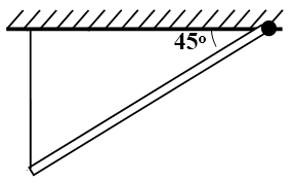
\includegraphics[scale=0.7]{../figs/VN10-PH-21-L-016-2-V2-02.png}
		\end{center}	
		
	}
	{\hide{
		Đầu tiên, ta quy định các đại lượng trong bài toán và xác định cánh tay đòn như sau: 
		\begin{itemize}
			\item $T$ là lực căng của sợi dây tác dụng lên điểm A trên tấm gỗ, 
			\item $P=m\cdot g= \left(\SI{30}{kg}\right)\cdot\left(\SI{10}{\meter/\second^2}\right) = \SI{300}{\newton}$ là trọng lực tác dụng lên tấm gỗ tại trọng tâm G, 
			\item $\alpha = 45^{\circ}$ là góc hợp bởi tấm gỗ và trần nhà, 
			\item $d$ là khoảng cách từ điểm G đến trục quay O,
			\item $d'$ là khoảng cách từ điểm treo của dây đến trục quay O,
			\item $l=\SI{1,8}{\meter}$ là chiều dài của thanh gỗ. 
		\end{itemize}
		%--------------------------------%
		\begin{center}
			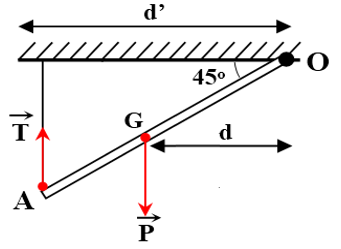
\includegraphics[scale=0.7]{../figs/VN10-PH-21-L-016-2-V2-03.png}
		\end{center}
		Cánh tay đòn của trọng lực:
		
		$$d=\si{OG}\cdot\cos 45^{\circ}.$$
		
		Cánh tay đòn tương ứng với lực căng dây là:
		
		$$d' = \si{OA}\cdot \cos 45^{\circ} .$$
		
		Áp dụng quy tắc moment lực:
		\begin{align*}
			T\cdot d' &= P\cdot d\\
			\Rightarrow
			T&=\dfrac{P\cdot d}{ d'}=\SI{200}{\newton}
		\end{align*}
		Vậy lực căng dây là $T=\SI{200}{\newton}$. 
	}}
	\viduii{3}{Thanh OA có khối lượng không đáng kể, có chiều dài $\SI{20}{\centi\meter}$, quay dễ dàng quanh trục nằm ngang O. Một lò xo gắn vào điểm giữa C. Người ta tác dụng vào đầu A của thanh một lực $F=\SI{200}{\newton}$ hướng thẳng đứng xuống dưới. Khi thanh ở trạng thái cân bằng, lò xo có hướng vuông góc với OA, OA hợp với đường thẳng nằm ngang một góc $\alpha=30^{\circ}$. Tìm phản lực N của lò xo lên thanh. 
		\begin{center}
			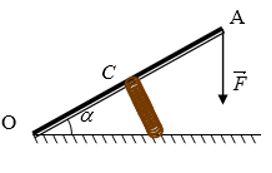
\includegraphics[scale=1]{../figs/VN10-PH-21-L-016-2-V2-04.png}
		\end{center}		
	}
	{\hide{
		Cánh tay đòn của lực $N$ là:
		
		$$\si{OC} = \dfrac{1}{2}\cdot \si{OA},$$
		
		do đoạn thẳng này vuông góc với giá của lực N. Cánh tay đòn tương ứng với lực $F$ là:
		
		$$\si{OB} = \si{OA}\cdot \cos\alpha.$$
		
		\begin{center}
			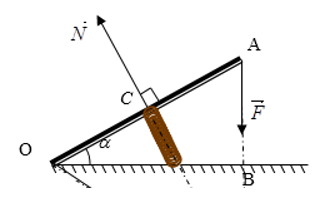
\includegraphics[scale=1]{../figs/VN10-PH-21-L-016-2-V2-05.png}
		\end{center}
		
		Áp dụng quy tắc moment lực:
		
		\begin{align*}
			&M_F=M_N\\
			\Rightarrow& F\cdot \si{OB} = N\cdot \si{OC}\\
			\Rightarrow& N  = \dfrac{F\cdot \si{OB}}{\si{OC}}
			=
			\dfrac{F\cdot \si{OA}\cdot \cos\alpha}{\dfrac{1}{2}\cdot \si{OA}}
			=2\cdot F\cdot \cos\alpha = \SI[parse-numbers=false]{200\sqrt{3}}{\newton}.
		\end{align*}
		%%%%
		Vậy phản lực tác dụng lên thanh có độ lớn là $N=\SI[parse-numbers=false]{200\sqrt{3}}{\newton}$.
		
	}}
	
\end{dang}
%\begin{dang}{Ghi nhớ khái niệm ngẫu lực, đặc điểm ngẫu lực}
%	\viduii{1}{Ngẫu lực là gì?
%		\begin{mcq}
%			\item Là hệ hai lực song song, cùng chiều.
%			\item Là hệ hai lực song song, ngược chiều.
%			\item Là hệ hai lực song song, cùng chiều có độ lớn bằng nhau và cùng tác dụng vào một vật.
%			\item Là hệ hai lực song song, ngược chiều có độ lớn bằng nhau và cùng tác dụng vào một vật.
%		\end{mcq}
%	}
%	{
%	\hide{	Ngẫu lực là hệ hai lực song song, ngược chiều có độ lớn bằng nhau và cùng tác dụng vào một vật.
%		
%		\textbf{Đáp án: D.}}
%	}
%	\viduii{1}{Chọn phát biểu sai	
%		\begin{mcq}
%			\item Tác dụng của ngẫu lực vào một vật làm cho vật quay và tịnh tiến.
%			\item Ngẫu lực là hệ hai lực song song, cùng chiều có độ lớn bằng nhau và cùng tác dụng vào một vật.
%			\item Đơn vị của ngẫu lực là $\SI{}{N\cdot m}$.
%			\item Cả A và B sai.
%		\end{mcq}	
%	}
%	{\hide{\begin{itemize}
%				\item Ngẫu lực là hệ hai lực song song, ngược chiều có độ lớn bằng nhau và cùng tác dụng vào một vật.
%				\item Tác dụng của ngẫu lực vào một vật chỉ làm cho vật quay chứ không tịnh tiến.
%				\item Đơn vị của ngẫu lực là $\SI{}{N\cdot m}$.
%			\end{itemize}
%			\textbf{Đáp án: D.}}
%	}
%\end{dang}
\begin{dang}{Tính moment ngẫu lực}
	\viduii{2}{Hai lực của một ngẫu lực có độ lớn $F= \SI{5,0}{\newton}$. Cánh tay đòn của ngẫu lực $d=\SI{20}{\centi\meter}$. Moment của ngẫu lực này là 
		\begin{mcq}(4)
			\item $\SI{10,0}{Nm}$.
			\item $\SI{2,0}{Nm}.$
			\item $\SI{0,5}{Nm}.$
			\item $\SI{1,0}{Nm}.$
		\end{mcq}		
	}
	{\hide{Moment ngẫu lực này là:
			
			$$M=F \cdot d= \SI{1,0}{Nm}.$$
			
			\textbf{Đáp án: D.}}
	}
\end{dang}